\documentclass{standalone}

\usepackage{pgfplots}

\begin{document}

\pgfplotsset{
colormap={whitered}{color(0cm)=(white); color(1cm)=(orange!75!red)},
colormap={whiteblue}{color(0cm)=(white); color(1cm)=(blue)},
}

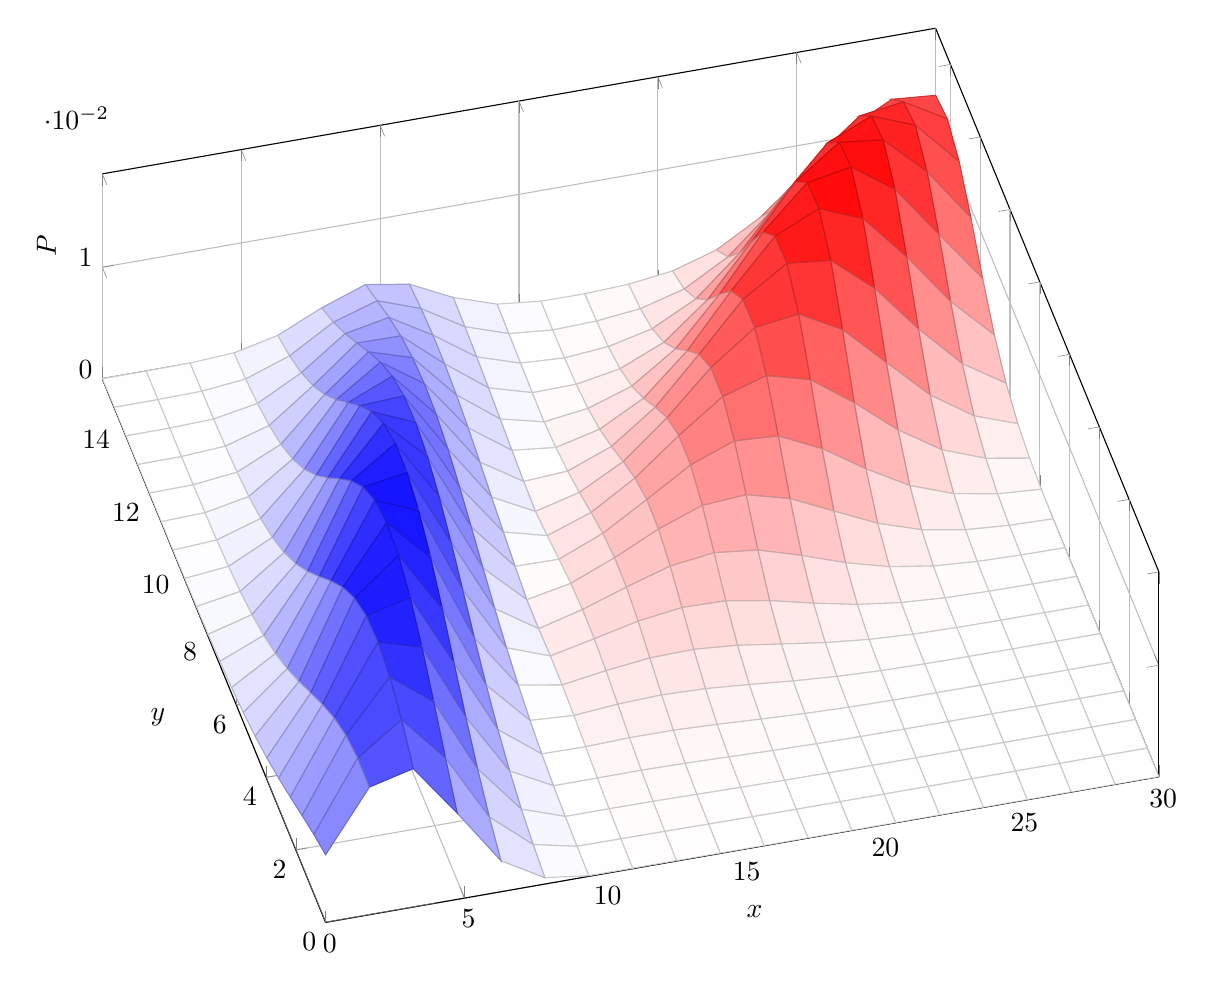
\begin{tikzpicture}[
    declare function={mu11=5;},
    declare function={mu12=5;},
    declare function={sigma11=3;},
    declare function={sigma12=5;},
    declare function={mu21=25;},
    declare function={mu22=12;},
    declare function={sigma21=5;},
    declare function={sigma22=3;},
    declare function={rho=0.8;},
    declare function={normal(\m,\s)=1/(2*\s*sqrt(pi))*exp(-(x-\m)^2/(2*\s^2));},
    declare function={bivar(\ma,\sa,\mb,\sb,\rho)=
        1/(2*pi*\sa*\sb*\rho) * exp(-((x-\ma)^2/\sa^2 + (y-\mb)^2/\sb^2 - (2*\rho*(x-\ma)*(y-\mb))/(\sa*\sb)))/(2*(1-\rho*\rho));}]
\begin{axis}[
    width=15cm,
    view={-15}{70},
    enlargelimits=false,
    grid=major,
    domain=0:30,
    y domain=0:15,
    samples=20,
    xlabel=$x$,
    ylabel=$y$,
    zlabel={$P$},
    %colorbar,
    colorbar style={
        at={(1.1,0)},
        anchor=south west,
        height=0.25*\pgfkeysvalueof{/pgfplots/parent axis height},
        title={$P(x_1,x_2)$}
    }
]
\addplot3 [
    surf,
    colormap={bluewhitered}{color(0cm)=(red); color(0.5cm)=(white); color(1cm)=(blue)},
    point meta={
    (
        bivar(mu11,sigma11,mu12,sigma12,rho)>
        bivar(mu21,sigma21,mu22,sigma22,rho)?
        bivar(mu11,sigma11,mu12,sigma12,rho):
        -bivar(mu21,sigma21,mu22,sigma22,rho)
    )   
    }
    ] {
    max(
        bivar(mu11,sigma11,mu12,sigma12,rho),
        bivar(mu21,sigma21,mu22,sigma22,rho)
    )};

\draw [black!50] (axis cs:-1,0,0) -- (axis cs:4,0,0);
\draw [black!50] (axis cs:0,-1,0) -- (axis cs:0,4,0);

\node at (axis cs:-1,1,0.18) [pin=165:$P(x_1)$] {};
\node at (axis cs:1.5,4,0.32) [pin=-15:$P(x_2)$] {};
\end{axis}
\end{tikzpicture}
\end{document}